\section{ĐỊNH LUẬT BOYLE}
\subsection{LÝ THUYẾT TRỌNG TÂM}
\subsubsection{Trạng thái và quá trình biến đổi trạng thái}
\begin{boxdn}
	\textbf{Trạng thái của một khối khí } được xác định bằng ba thông số, gọi là thông số trạng thái của khối khí: thể tích $V$, áp suất $p$ và nhiệt độ tuyệt đối $T$. Giữa các thông số trạng thái của một khối khí xác định có những mối liên hệ mang tính quy luật.
\end{boxdn}
\begin{center}
	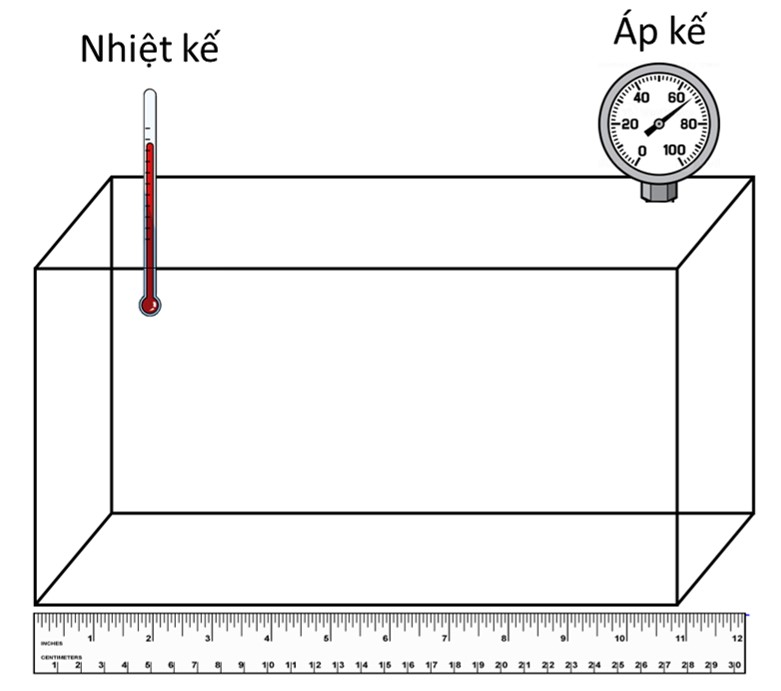
\includegraphics[width=0.35\linewidth]{figs/VN12-Y24-PH-SYL-010-1}
	\captionof{figure}{Xác định các thông số trạng thái của một lượng khí}
\end{center}
\begin{boxdn}
	\textbf{Quá trình biến đổi trạng thái là} quá trình khối khí biến đổi từ trạng thái này sang trạng thái khác.\\
	\textbf{Đẳng quá trình} là quá trình biến đổi trạng thái mà trong đó có một thông số trạng thái được giữ không đổi.\\
	Các đẳng quá trình:
	\begin{itemize}
		\item Đẳng nhiệt là quá trình biến đổi trạng thái của một khối khí xác định, trong đó nhiệt độ được giữ không đổi.
		\item Đẳng áp là quá trình biến đổi trạng thái của một khối khí xác định, trong đó áp suất được giữ không đổi.
		\item Đẳng tích là quá trình biến đổi trạng thái của một khối khí xác định, trong đó thể tích được giữ không đổi.
	\end{itemize}
\end{boxdn}
\begin{luuy}
	Vì chất khí luôn chiếm toàn bộ dung tích của bình chứa nên thể tích của một lượng khí bằng dung tích bình chứa nó.
\end{luuy}
\subsubsection{Định luật Boyle}
\begin{boxdl}
	Ở nhiệt độ không đổi, áp suất của một khối khí xác định tỉ lệ nghịch với thể tích của nó.
	\begin{equation}
		pV=\text{hằng số}
	\end{equation}
\end{boxdl}
Đường biểu diễn sự phụ thuộc của $p$ theo $V$ khi nhiệt độ của khối khí không đổi gọi là \textbf{đường đẳng nhiệt}.
\begin{center}
	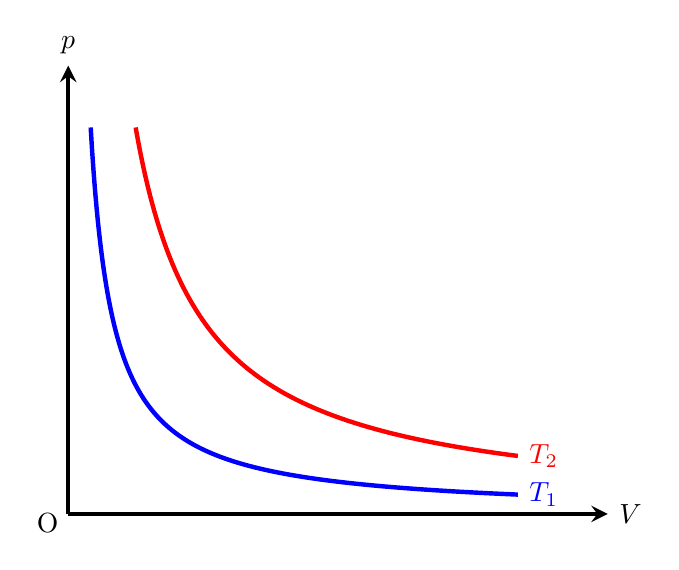
\begin{tikzpicture}  
		\begin{axis}[  ultra thick,
			xmin=0,  
			xmax=24,  
			xtick=\empty,
			ytick=\empty,
			ymin=0,  
			ymax=5.8, 
			samples=300,
			xticklabels=\empty,
			yticklabels=\empty,
			axis lines=center, 
			xlabel=$V$, 
			ylabel=$p$, 
			every axis y label/.style={at=(current axis.above origin),anchor=south},  
			every axis x label/.style={at=(current axis.right of origin),anchor=west},  ]
			\addplot [ultra thick, blue, smooth, domain=1:20] {5/x} node[right] {$T_1$}; 
			\addplot [ultra thick, red, smooth, domain=3:20] {15/x} node[right] {$T_2$}; 
		\end{axis}  
		\node[label={[below left]90:O}] at (0,0){};
	\end{tikzpicture}
	\captionof{figure}{Các đường đẳng nhiệt của một khối khí lí tưởng tương ứng với nhiệt độ $T_1$ và $T_2\left(T_2>T_1\right)$}
	
\end{center}
\subsection{Mục tiêu bài học - Ví dụ minh hoạ}
\begin{dang}{Vận dụng định luật Boyle giải thích được một số hiện tượng trong thực tế}
	\end{dang}
\begin{vd}
Nếu lật úp một chiếc cốc thuỷ tinh rồi nhúng chìm chiếc cốc vào trong nước thì thể tích phần không khí bị giam trong cốc sẽ thay đổi như thế nào trong quá trình chiếc cốc chìm sâu xuống nước?
\loigiai{
			Trong quá trình cốc chìm xuống nước thì nhiệt độ không khí trong cốc không thay đổi. Cốc càng chìm sâu vào trong nước thì áp suất của không khí trong cốc càng tăng. Theo định luật Boyle, khi đó thể tích của không khí bị giam trong cốc ngày càng giảm.
}
\end{vd}
% ======================================================
\begin{vd}
Để đưa thuốc từ lọ vào trong cylanh của ống tiêm, ban đầu nhân viên y tế đẩy piston sát đáy cylanh, sau đó đưa đầu kim tiêm (được gắn với ống tiêm) vào trong lọ thuốc. Khi kéo piston, thuốc sẽ chảy vào trong cylanh. Em hãy giải thích cơ sở khoa học của việc làm trên?
	\begin{center}
		
\includegraphics[width=0.35\linewidth]{figs/VN12-Y24-PH-SYL-010-2}
	\end{center}
\loigiai{
		Khi mới đưa đầu kim tiêm vào trong lọ thuốc, áp suất khí còn lại trong cylanh bằng áp suất chất lỏng trong lo thuốc. Khi kéo piston, thể tích khí trong cylanh tăng (nhiệt độ khí gần như không đổi). Theo định luật Boyle, áp suất khí trong cylanh giảm và nhỏ hơn áp suất chất lỏng trong lọ. Do đó, chất lỏng trong lọ bị đẩy qua kim và chảy sang cylanh cho đến khi có sự cân bằng áp suất ở cả hai phía.
	}
\end{vd}

\begin{dang}{Giải được các bài toán liên quan quá trình đẳng nhiệt}
\end{dang}
\begin{vd}
Một lượng khí có thể tích $\SI{10}{\text{lít}}$ ở áp suất $\SI{E5}{\pascal}$. Tính thể tích của lượng khí này ở áp suất $\SI{1.25E5}{\pascal}$. Biết nhiệt độ của khí không đổi.
\loigiai{
		\begin{center}
			\begin{tabular}{C{4cm} C{3cm} C{4cm}}
				\colorbox{yellow}{\textcolor{red}{\textbf{Trạng thái 1}}} & $\xrightarrow[]{T_1=T_2}$ & \colorbox{yellow}{\textcolor{red}{\textbf{Trạng thái 2}}}\\
				$p_1=\SI{E5}{\pascal}$ & &$p_2=\SI{1.25E5}{\pascal}$\\
				$V_1=\SI{10}{\text{lít}}$ & & $V_2=?$
			\end{tabular}
		\end{center}
		Theo định luật Boyle:
		$$p_1V_1=p_2V_2\Rightarrow V_2=\dfrac{p_1V_1}{p_2}=\dfrac{\left(\SI{E5}{\pascal}\right)\cdot\left(\SI{10}{\text{lít}}\right)}{\SI{1.25E5}{\pascal}}=\SI{8}{\text{lít}}.$$
		Vậy: ở áp suất $\SI{1.25E5}{\pascal}$ thì thể tích bọt khí là $\SI{8}{\text{lít}}$.
}
\end{vd}
% ===============================================================	
\begin{vd}
Một bọt khí nổi lên từ đáy giếng sâu $\SI{6}{\meter}$ lên mặt nước. Khi lên tới mặt nước, thể tích của bọt khí tăng lên bao nhiêu lần? Coi áp suất khí quyển là $\SI{1.013E5}{\pascal}$; khối lượng riêng của nước giếng là $\SI{1003}{\kilogram/\meter^3}$ và nhiệt độ của nước giếng không thay đổi theo độ sâu. Lấy gia tốc trọng trường $g=\SI{9.81}{\meter/\second^2}$.
\loigiai{
		Áp suất trong bọt khí khi ở độ sâu $\SI{6}{\meter}$ so với mặt nước:
		$$p_1=p_0+\rho gh=\SI{1.013E5}{\pascal}+\left(\SI{1003}{\kilogram/\meter^3}\right)\cdot\left(\SI{9.81}{\meter
			/\second^2}\right)\cdot\left(\SI{6}{\meter}\right)\approx\SI{1.6E5}{\pascal}$$
		\begin{center}
			\begin{tabular}{C{4cm} C{3cm} C{4cm}}
				\colorbox{yellow}{\textcolor{red}{\textbf{Trạng thái 1}}} & $\xrightarrow[]{T_1=T_2}$ & \colorbox{yellow}{\textcolor{red}{\textbf{Trạng thái 2}}}\\
				$p_1=\SI{1.6E5}{\pascal}$ & &$p_2=p_0=\SI{1.013E5}{\pascal}$\\
				$V_1$ & & $V_2$
			\end{tabular}
		\end{center}
		Theo định luật Boyle:
		$$p_1V_1=p_2V_2\Rightarrow \dfrac{V_2}{V_1}=\dfrac{p_1}{p_2}=\dfrac{\SI{1.6E5}{\pascal}}{\SI{1.013E5}{\pascal}}\approx1,58.$$
		Vậy: khi nổi lên mặt nước, thể tích bọt khí đã tăng lên 1,58 lần.
}
\end{vd}
% ==============================================================
\begin{vd}
	Một cột không khí chứa trong một ống nhỏ, dài, tiết diện đều, ban đầu ống được đặt nằm ngang (như hình). Cột không khí được ngăn cách bởi một cột thuỷ ngân có chiều dài $d=\SI{150}{\milli\meter}$. Áp suất khí quyển là $p_0=\SI{750}{\milli\meter Hg}$. Biết chiều dài ban đầu của cột không khí là $\ell_0=\SI{144}{\milli\meter}$.
		\begin{center}
			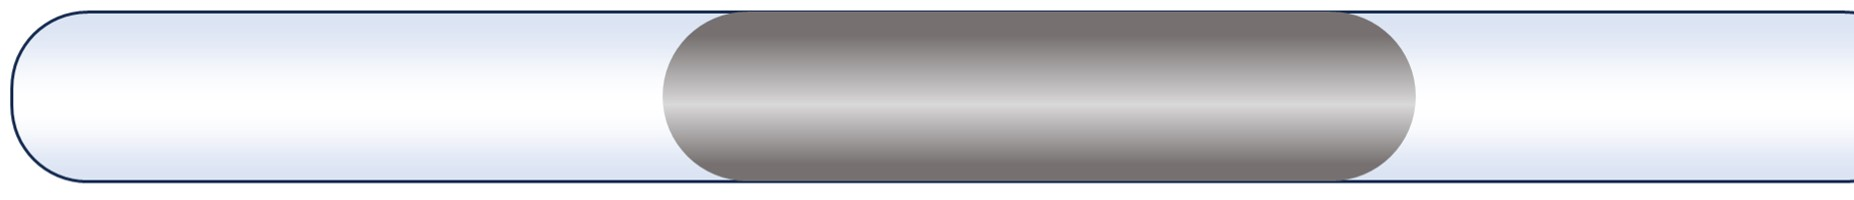
\includegraphics[width=0.4\linewidth]{figs/VN12-Y24-PH-SYL-010-3}
		\end{center}
		Hãy tính chiều dài cột không khí nếu:
		\begin{enumerate}[label=\alph*)]
			\item ống thẳng đứng, miệng ống ở trên.
			\item ống thẳng đứng, miệng ống ở dưới.
			\item ống đặt nghiêng góc $\alpha=\SI{30}{\degree}$ so với phương ngang, miệng ống ở dưới.
			\item ống đặt nghiêng góc $\alpha=\SI{30}{\degree}$ so với phương ngang, miệng ống ở trên.
		\end{enumerate}
		Giả sử ống đủ dài để cột thuỷ ngân luôn ở trong ống và nhiệt độ là không đổi.
	\loigiai{Gọi $S$ là tiết diện của ống.
			\begin{enumerate}[label=\alph*)]
				\item Trường hợp ống đặt thẳng đứng, miệng ống hướng lên:\\
				\begin{minipage}[l]{0.25\textwidth}
					\begin{center}
						
\includegraphics[width=0.1\linewidth]{figs/VN12-Y24-PH-SYL-010-4}
					\end{center}
				\end{minipage}
				\begin{minipage}[l]{0.75\textwidth}
					\begin{center}
						\begin{tabular}{C{4cm} C{2cm} C{4cm}}
							\colorbox{yellow}{\textcolor{red}{\textbf{Trạng thái ban đầu}}} & $\xrightarrow[]{T=const}$ & \colorbox{yellow}{\textcolor{red}{\textbf{Trạng thái câu a}}}\\
							$p_0=\SI{750}{\milli\meter Hg}$ & &$p_a=p_0+d=\SI{900}{\milli\meter Hg}$\\
							$V_0=\ell_0S$ & & $V_a=\ell_a S$
						\end{tabular}
					\end{center}
					Theo định luật Boyle:
					$$p_0V_0=p_aV_a$$
					$$\Leftrightarrow p_0\ell_0S=p_a\ell_aS$$
					$$\Rightarrow \ell_a=\dfrac{p_0\ell_0}{p_a}=\dfrac{\left(\SI{750}{\milli\meter Hg}\right)\cdot\left(\SI{144}{\milli\meter}\right)}{\SI{900}{\milli\meter Hg}}=\SI{120}{\milli\meter}.$$
				\end{minipage}
				\item Trường hợp ống đặt thẳng đứng, miệng ống hướng xuống:\\
				\begin{minipage}[l]{0.25\textwidth}
					\begin{center}
						
\includegraphics[width=0.1\linewidth]{figs/VN12-Y24-PH-SYL-010-5}
					\end{center}
				\end{minipage}
				\begin{minipage}[l]{0.75\textwidth}
					\begin{center}
						\begin{tabular}{C{4cm} C{2cm} C{4cm}}
							\colorbox{yellow}{\textcolor{red}{\textbf{Trạng thái ban đầu}}} & $\xrightarrow[]{T=const}$ & \colorbox{yellow}{\textcolor{red}{\textbf{Trạng thái câu b}}}\\
							$p_0=\SI{750}{\milli\meter Hg}$ & &$p_b=p_0-d=\SI{600}{\milli\meter Hg}$\\
							$V_0=\ell_0S$ & & $V_b=\ell_b S$
						\end{tabular}
					\end{center}
					Theo định luật Boyle:
					$$p_0V_0=p_bV_b$$
					$$\Leftrightarrow p_0\ell_0S=p_b\ell_bS$$
					$$\Rightarrow \ell_b=\dfrac{p_0\ell_0}{p_b}=\dfrac{\left(\SI{750}{\milli\meter Hg}\right)\cdot\left(\SI{144}{\milli\meter}\right)}{\SI{600}{\milli\meter Hg}}=\SI{180}{\milli\meter}.$$
				\end{minipage}
				\item Trường hợp ống đặt nghiêng góc $\alpha=\SI{30}{\degree}$ so với phương ngang, miệng ống ở dưới:\\
				\begin{minipage}[l]{0.25\textwidth}
					\begin{center}
						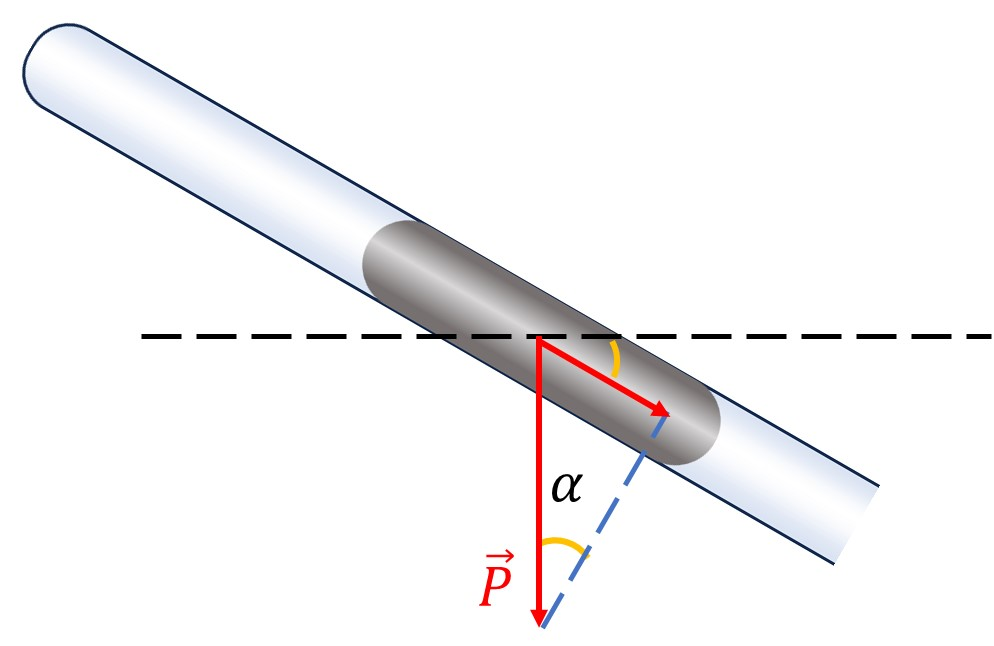
\includegraphics[width=1.0\linewidth]{figs/VN12-Y24-PH-SYL-010-6}
					\end{center}
				\end{minipage}
				\begin{minipage}[l]{0.75\textwidth}
					\begin{center}
						\begin{tabular}{C{4cm} C{1.5cm} C{4.5cm}}
							\colorbox{yellow}{\textcolor{red}{\textbf{Trạng thái ban đầu}}} & $\xrightarrow[]{T=const}$ & \colorbox{yellow}{\textcolor{red}{\textbf{Trạng thái câu c}}}\\
							$p_0=\SI{750}{\milli\meter Hg}$ & &$p_c=p_0-d\sin\alpha=\SI{675}{\milli\meter Hg}$\\
							$V_0=\ell_0S$ & & $V_c=\ell_c S$
						\end{tabular}
					\end{center}
					Theo định luật Boyle:
					$$p_0V_0=p_cV_c$$
					$$\Leftrightarrow p_0\ell_0S=p_c\ell_cS$$
					$$\Rightarrow \ell_c=\dfrac{p_0\ell_0}{p_c}=\dfrac{\left(\SI{750}{\milli\meter Hg}\right)\cdot\left(\SI{144}{\milli\meter}\right)}{\SI{675}{\milli\meter Hg}}=\SI{160}{\milli\meter}.$$
				\end{minipage}
				\item Trường hợp ống đặt nghiêng góc $\alpha=\SI{30}{\degree}$ so với phương ngang, miệng ống ở trên:\\
				\begin{minipage}[l]{0.25\textwidth}
					\begin{center}
						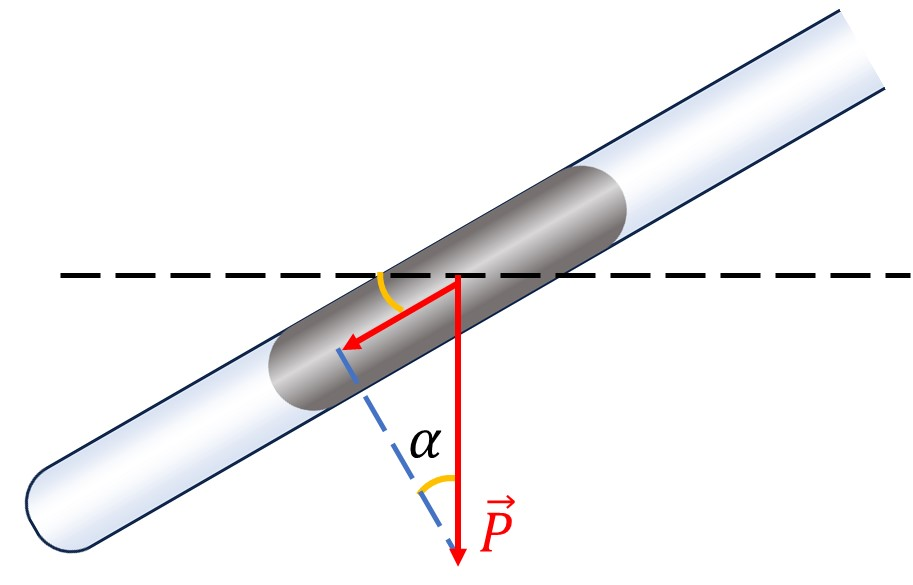
\includegraphics[width=1.0\linewidth]{figs/VN12-Y24-PH-SYL-010-7}
					\end{center}
				\end{minipage}
				\begin{minipage}[l]{0.75\textwidth}
					\begin{center}
						\begin{tabular}{C{4cm} C{1.5cm} C{4.5cm}}
							\colorbox{yellow}{\textcolor{red}{\textbf{Trạng thái ban đầu}}} & $\xrightarrow[]{T=const}$ & \colorbox{yellow}{\textcolor{red}{\textbf{Trạng thái câu d}}}\\
							$p_0=\SI{750}{\milli\meter Hg}$ & &$p_d=p_0+d\sin\alpha=\SI{825}{\milli\meter Hg}$\\
							$V_0=\ell_0S$ & & $V_d=\ell_d S$
						\end{tabular}
					\end{center}
					Theo định luật Boyle:
					$$p_0V_0=p_dV_d$$
					$$\Leftrightarrow p_0\ell_0S=p_d\ell_dS$$
					$$\Rightarrow \ell_d=\dfrac{p_0\ell_0}{p_d}=\dfrac{\left(\SI{750}{\milli\meter Hg}\right)\cdot\left(\SI{144}{\milli\meter}\right)}{\SI{825}{\milli\meter Hg}}\approx\SI{131}{\milli\meter}.$$
				\end{minipage}
			\end{enumerate}
	}
\end{vd}
\begin{dang}{Giải được bài toán piston cân bằng}
	\end{dang}
\begin{vd}
	Một lượng không khí có thể tích $\SI{240}{\centi\meter^3}$ chứa trong một cylanh có piston đóng kín, tiết diện của piston là $\SI{24}{\centi\meter^2}$. Áp suất của không khí trong cylanh bằng áp suất không khí bên ngoài là $\SI{E5}{\pascal}$. Cần một lực tối thiểu bằng bao nhiêu để dịch chuyển piston một đoạn $\SI{2}{\centi\meter}$ theo chiều làm thể tích khí giảm? Bỏ qua ma sát giữa giữa piston và thành cylanh. Coi trong quá trình piston chuyển động thì nhiệt độ của không khí không thay đổi.
	\begin{center}
		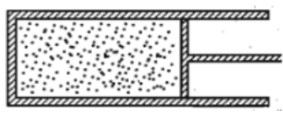
\includegraphics[width=0.25\linewidth]{figs/VN12-Y24-PH-SYL-010-8}
	\end{center}
\loigiai{
	\begin{center}
		\begin{tabular}{C{6cm} C{2cm} C{7cm}}
			\colorbox{yellow}{\textcolor{red}{\textbf{Trạng thái 1}}} & $\xrightarrow[]{T_1=T_2}$ & \colorbox{yellow}{\textcolor{red}{\textbf{Trạng thái 2}}}\\
			$p_1=\SI{E5}{\pascal}$ & &$p_2=?$\\
			$V_1=\SI{240}{\centi\meter^3}$ & & $V_2=\SI{240}{\centi\meter^3}-\left(\SI{24}{\centi\meter^2}\right)\cdot\left(\SI{2}{\centi\meter}\right)=\SI{192}{\centi\meter^3}$
		\end{tabular}
	\end{center}
	Theo định luật Boyle:
	$$p_1V_1=p_2V_2\Rightarrow p_2=\dfrac{p_1V_1}{V_2}=\dfrac{\left(\SI{100}{\kilo\pascal}\right)\cdot\left(\SI{240}{\centi\meter^3}\right)}{\SI{192}{\centi\meter^3}}=\SI{125}{\kilo\pascal}.$$
	\begin{center}
		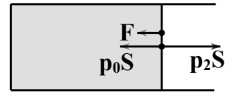
\includegraphics[width=0.25\linewidth]{figs/VN12-Y24-PH-SYL-010-9}
	\end{center}
	Piston cân bằng khi:
	$$p_2S=p_0S+F\Rightarrow F=\left(p_2-p_0\right)S=\left(\SI{125E3}{\pascal}-\SI{100E3}{\pascal}\right)\cdot\left(\SI{24E-4}{\meter^2}\right)=\SI{60}{\newton}.$$
}
\end{vd}
% ===============================================================
\begin{vd}
	Một bình hình trụ kín hai đầu có độ cao $h=\SI{40}{\centi\meter}$, được đặt nằm ngang, bên trong có một piston rất mỏng và có thể dịch chuyển không ma sát trong bình. Lúc đầu piston được giữ cố định ở chính giữa bình. Hai bên piston chứa cùng loại khí nhưng áp suất khí bên trái $\left(p_1\right)$ lớn gấp 3 lần áp suất khí chứa ở bên phải $\left(p_2\right)$. Piston và thành bình đều được làm từ vật liệu cách nhiệt. Khi thả để piston di chuyển tự do thì piston sẽ di chuyển một đoạn bao nhiêu, theo chiều nào?
		\begin{center}
			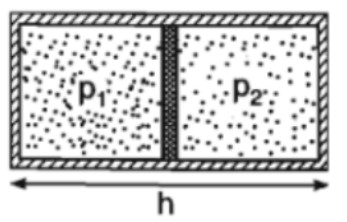
\includegraphics[width=0.25\linewidth]{figs/VN12-Y24-PH-SYL-010-10}
		\end{center}
\loigiai{
			Vì áp suất khí bên trái lớn hơn áp suất khí bên phải nên khi được thả tự do piston sẽ di chuyển theo chiều từ trái sang phải.\\
			Piston di chuyển đến khi áp suất khí hai bên piston cân bằng. Gọi:
			\begin{itemize}
				\item $p$ là áp suất khí mỗi bên khi piston đạt trạng thái cân bằng;
				\item $x$ là độ dời của piston.
			\end{itemize}
			Áp dụng định luật Boyle cho khí ở mỗi vách ngăn khi vừa thả piston và khi piston cân bằng:
			$$pV=\text{const}\Rightarrow \begin{cases}
				p_1\cdot\dfrac{hS}{2}=p\left(\dfrac{h}{2}+x\right)S\\
				p_2\cdot\dfrac{hS}{2}=p\left(\dfrac{h}{2}-x\right)S\\
			\end{cases}\Rightarrow \dfrac{p_1}{p_2}=\dfrac{\SI{20}{\centi\meter}+x}{\SI{20}{\centi\meter}-x}=3\Rightarrow x=\SI{10}{\centi\meter}.$$
			
	}
\end{vd}
\subsection{BÀI TẬP TRẮC NGHIỆM}
\Opensolutionfile{ans}[ans/G12Y24B9TN]
% ===================================================================
\begin{ex}
	Tập hợp ba thông số xác định trạng thái của một lượng khí xác định là
	\choice
	{áp suất, thể tích, khối lượng}
	{\True áp suất, nhiệt độ, thể tích}
	{thể tích, trọng lượng, áp suất}
	{áp suất, nhiệt độ, số mol}
	\loigiai{}
\end{ex}
% ===================================================================
\begin{ex}
	Quá trình đẳng nhiệt là
	
	\choice
	{quá trình biến đổi trạng thái của một lượng khí xác định trong đó áp suất được giữ không đổi}
	{quá trình biến đổi trạng thái của một lượng khí xác định trong đó nội năng của khí không đổi}
	{\True quá trình biến đổi trạng thái của một lượng khí xác định trong đó nhiệt độ được giữ không đổi}
	{quá trình biến đổi trạng thái của một lượng khí xác định trong đó thể tích được giữ không đổi}
	\loigiai{}
\end{ex}
% ===================================================================
\begin{ex}
	Trong các hệ thức sau đây, hệ thức nào \textbf{không phù hợp} với định luật Boyle?
	\choice
	{$p\sim\dfrac{1}{V}$}
	{$pV=\text{const}$}
	{\True $V\sim p$}
	{$p_1V_1=p_2V_2$}
	\loigiai{}
\end{ex}
% ===================================================================
\begin{ex}
Nhận định nào sau đây là \textbf{sai} khi nói về quá trình đẳng nhiệt?	
	\choice
	{Tích của áp suất và thể tích luôn không đổi}
	{Áp suất và thể tích tỉ lệ nghịch với nhau}
	{Khi áp suất khí tăng 2 lần thì tích $pV$ vẫn không đổi}
	{\True Khi thể tích khí giảm 2 lần thì áp suất khí cũng giảm 2 lần}
	\loigiai{}
\end{ex}
% ===================================================================
\begin{ex}
Đường đẳng nhiệt trong hệ trục toạ độ $pOV$ là
	
	\choice
	{đường thẳng đi qua gốc toạ độ}
	{đường thẳng kéo dài đi qua gốc toạ độ}
	{\True đường cong hyperbol}
	{một nhánh của parabol}
	\loigiai{}
\end{ex}
% ===================================================================
\begin{ex}
	Cho một lượng khí lí tưởng xác định. Nén đẳng nhiệt khối khí từ thể tích $\SI{10}{\liter}$ đến thể tích $\SI{4}{\liter}$ thì áp suất khí
	\choice
	{\True tăng 2,5 lần}
	{giảm 2,5 lần}
	{tăng 6 lần}
	{giảm 6 lần}
	\loigiai{$$p_1V_1=p_2V_2\Rightarrow\dfrac{p_2}{p_1}=\dfrac{V_1}{V_2}=2,5.$$
	}
\end{ex}
% ===================================================================
\begin{ex}
	Một lượng khí lí tưởng xác định dãn nở đẳng nhiệt từ thể tích $\SI{2}{\liter}$ đến $\SI{8}{\liter}$, ban đầu áp suất khí là $\SI{8E5}{\pascal}$. Trong quá trình trên thì áp suất khí
	\choice
	{tăng $\SI{6E5}{\pascal}$}
	{tăng $\SI{2E5}{\pascal}$}
	{giảm $\SI{2E5}{\pascal}$}
	{\True giảm $\SI{6E5}{\pascal}$}
	\loigiai{$$p_2=\dfrac{p_1V_1}{V_2}=\SI{2E5}{\pascal}\Rightarrow \Delta p=p_2-p_1=\SI{-6E5}{\pascal}.$$
	}
\end{ex}
% ===================================================================
\begin{ex}
	Nén đẳng nhiệt một khối khí lí tưởng xác định làm áp suất khí thay đổi một lượng $\SI{0.5}{atm}$. Biết thể tích và áp suất ban đầu của khối khí là $\SI{5}{\liter}$ và $\SI{2}{atm}$. Thể tích của khối khí lúc sau là
	\choice
	{$\SI{6.25}{\liter}$}
	{\True $\SI{4}{\liter}$}
	{$\SI{6.67}{\liter}$}
	{$\SI{20}{\liter}$}
	\loigiai{\begin{center}
			\begin{tabular}{C{4cm} C{3cm} C{4cm}}
				\colorbox{yellow}{\textcolor{red}{\textbf{Trạng thái 1}}} & $\xrightarrow[]{T_1=T_2}$ & \colorbox{yellow}{\textcolor{red}{\textbf{Trạng thái 2}}}\\
				$p_1=\SI{2}{atm}$ & &$p_2=\SI{2.5}{atm}$\\
				$V_1=\SI{5}{\liter}$ & & $V_2=?$
			\end{tabular}
		\end{center}
		Vì thể tích khí giảm nên áp suất khí tăng.\\
		$$V_2=\dfrac{p_1V_1}{p_2}=\SI{4}{\liter}.$$
	}
\end{ex}
% ===================================================================
\begin{ex}
	Khi thở ra dung tích của phổi là $\SI{2.4}{\liter}$ và áp suất của không khí trong phổi là $\SI{101.7}{\kilo\pascal}$. Khi hít vào áp suất của phổi là $\SI{101.01}{\kilo\pascal}$. Coi nhiệt độ của phổi là không đổi, dung tích của phổi khi hít vào bằng
	
	\choice
	{\True $\SI{2.416}{\liter}$}
	{$\SI{2.384}{\liter}$}
	{$\SI{2.4}{\liter}$}
	{$\SI{1.327}{\liter}$}
	\loigiai{\begin{center}
			\begin{tabular}{C{4cm} C{3cm} C{4cm}}
				\colorbox{yellow}{\textcolor{red}{\textbf{Trạng thái 1}}} & $\xrightarrow[]{T_1=T_2}$ & \colorbox{yellow}{\textcolor{red}{\textbf{Trạng thái 2}}}\\
				$p_1=\SI{101.7}{\kilo\pascal}$ & &$p_2=\SI{101.01}{\kilo\pascal}$\\
				$V_1=\SI{2.4}{\liter}$ & & $V_2=?$
			\end{tabular}
		\end{center}
		Theo định luật Boyle:
		$$p_1V_1=p_2V_2\Rightarrow V_2=\SI{2.416}{\liter}.$$
	}
\end{ex}
% ===================================================================
\begin{ex}
	Một khối khí lí tưởng xác định có áp suất $\SI{1}{atm}$ được nén đến áp suất $\SI{4}{atm}$ ở nhiệt độ không đổi thì thể tích biến đổi một lượng $\SI{3}{\liter}$. Thể tích ban đầu của khối khí đó là
	\choice
	{\True $\SI{4}{\liter}$}
	{$\SI{1}{\liter}$}
	{$\SI{0.75}{\liter}$}
	{$\SI{12}{\liter}$}
	\loigiai{\begin{center}
			\begin{tabular}{C{4cm} C{3cm} C{4cm}}
				\colorbox{yellow}{\textcolor{red}{\textbf{Trạng thái 1}}} & $\xrightarrow[]{T_1=T_2}$ & \colorbox{yellow}{\textcolor{red}{\textbf{Trạng thái 2}}}\\
				$p_1=\SI{1}{atm}$ & &$p_2=\SI{4}{atm}$\\
				$V_1=?$ & & $V_2=V_1-\SI{3}{\liter}$
			\end{tabular}
		\end{center}
		$$p_1V_1=p_2V_2\Rightarrow V_1=\SI{4}{\liter}.$$
	}
\end{ex}
% ===================================================================
\begin{ex}
	Nếu áp suất của một lượng khí lí tưởng xác định tăng $\SI{2E5}{\pascal}$ thì thể tích biến đổi $\SI{3}{\liter}$. Nếu áp suất của lượng khí đó tăng $\SI{5E5}{\pascal}$ thì thể tích biến đổi $\SI{5}{\liter}$. Biết nhiệt độ khí không đổi. Áp suất và thể tích ban đầu của khí là
	\choice
	{$\SI{2E5}{\pascal}$, $\SI{8}{\liter}$}
	{$\SI{4E5}{\pascal}$, $\SI{12}{\liter}$}
	{\True $\SI{4E5}{\pascal}$, $\SI{9}{\liter}$}
	{$\SI{2E5}{\pascal}$, $\SI{12}{\liter}$}
	\loigiai{\begin{center}
			\begin{tabular}{C{3.5cm} C{2.0cm} C{3.5cm} C{2.0cm} C{3.5cm}}
				\colorbox{yellow}{\textcolor{red}{\textbf{Trạng thái 2}}}& $\xleftarrow[]{T_1=T_2}$ & \colorbox{yellow}{\textcolor{red}{\textbf{Trạng thái 1}}} &$\xrightarrow[]{T_1=T_3}$ & \colorbox{yellow}{\textcolor{red}{\textbf{Trạng thái 3}}}\\
				$p_2=p_1+\SI{2E5}{\pascal}$	 & &$p_1=?$ & &$p_3=p_1+\SI{5E5}{\pascal}$\\
				$V_2=V_1-\SI{3}{\liter}$ & & $V_1=?$ & & $V_3=V_1-\SI{5}{\liter}$
			\end{tabular}
		\end{center}
		$$pV=\text{const}\Rightarrow\begin{cases}
			p_1V_1=\left(p_1+\SI{2E5}{}\right)\cdot\left(V_1-3\right)\\
			p_1V_1=\left(p_1+\SI{5E5}{}\right)\cdot\left(V_1-5\right)
		\end{cases}\Rightarrow \begin{cases}
			3p_1-\SI{2E5}{}V_1=\SI{-6E5}{}\\
			5p_1-\SI{5E5}{}V_1=\SI{-25E5}{}\\
		\end{cases}\Rightarrow \begin{cases}
			p_1=\SI{4E5}{\pascal}\\
			V_1=\SI{9}{\liter}
		\end{cases}.$$}
\end{ex}
% ===================================================================
\begin{ex}
Người ta bơm không khí ở áp suất $\SI{1}{atm}$ vào bình có dung tích $\SI{10}{\liter}$. Biết mỗi lần bơm thì bơm được $\SI{250}{\centi\meter^3}$ không khí. Trước khi bơm đã có không khí $\SI{1}{atm}$ trong bình và nhiệt độ khí trong quá trình bơm không đổi. Áp suất khí sau 50 lần bơm là	
	\choice
	{$\SI{1.45}{atm}$}
	{$\SI{4.25}{atm}$}
	{$\SI{2.85}{atm}$}
	{\True $\SI{2.25}{atm}$}
	\loigiai{\begin{center}
			\begin{tabular}{C{4cm} C{3cm} C{4cm}}
				\colorbox{yellow}{\textcolor{red}{\textbf{Trạng thái trước khi bơm}}} & $\xrightarrow[]{T_1=T_2}$ & \colorbox{yellow}{\textcolor{red}{\textbf{Trạng thái sau khi bơm}}}\\
				$p_1=\SI{1}{atm}$ & &$p_2=?$\\
				$V_1=10+0,25\cdot50=\SI{22.5}{\liter}$ & & $V_2=\SI{10}{\liter}$
			\end{tabular}
		\end{center}
		$$p_1V_1=p_2V_2\Rightarrow p_2=\dfrac{p_1V_1}{V_2}=\SI{2.25}{atm}.$$
	}
\end{ex}
% ===================================================================
\begin{ex}
Sử dụng một cái bơm để bơm không khí vào quả bóng đá có bán kính khi bơm căng là $\SI{11}{\centi\meter}$. Mỗi lần bơm đưa được $\SI{0.32}{\liter}$ khí ở điều kiện $\SI{1}{atm}$ vào bóng. Giả thiết rằng quả bóng trước khi bơm không có không khí và nhiệt độ không đổi trong quá trình bơm. Sau 35 lần bơm thì áp suất khí bên trong quả bóng là	
	\choice
	{\True $\SI{2.0}{atm}.$}
	{$\SI{2.1}{atm}.$}
	{$\SI{0.7}{atm}.$}
	{$\SI{2.9}{atm}.$}
	\loigiai{\begin{center}
			\begin{tabular}{C{4cm} C{3cm} C{4cm}}
				\colorbox{yellow}{\textcolor{red}{\textbf{Trạng thái trước khi bơm}}} & $\xrightarrow[]{T_1=T_2}$ & \colorbox{yellow}{\textcolor{red}{\textbf{Trạng thái sau khi bơm}}}\\
				$p_1=\SI{1}{atm}$ & &$p_2=?$\\
				$V_1=35\cdot\left(\SI{0.32}{\liter}\right)=\SI{11.2}{\liter}$ & & $V_2=\dfrac{4}{3}\pi r^3\approx\SI{5.58}{\liter}$
			\end{tabular}
		\end{center}
		$$p_1V_1=p_2V_2\Rightarrow p_2=\dfrac{p_1V_1}{V_2}=\SI{2.0}{atm}.$$
	}
\end{ex}
% ===================================================================
\begin{ex}
	Một học sinh dùng bơm tay để bơm không khí vào một quả bóng cao su có thể tích $\SI{3}{\liter}$ với áp suất không khí là $\SI{E5}{\pascal}$. Xung quanh của bơm có chiều cao là $\SI{42}{\centi\meter}$, đường kính cylanh là $\SI{5}{\centi\meter}$. Trước khi bơm thì bên trong quả bóng đã có không khí với áp suất $\SI{E5}{\pascal}$ và xem như nhiệt độ không đổi trong quá trình bơm. Để không khí trong bóng đạt áp suất $\SI{5E5}{\pascal}$ thì học sinh đó phải bơm
	\choice
	{6 lần}
	{16 lần}
	{\True 15 lần}
	{10 lần}
	\loigiai{Thể tích lượng khí của mỗi lần bơm vào bóng:
		$$\Delta V=\pi r^2 h=\xsi{0,2625\pi}{\liter}.$$
		\begin{center}
			\begin{tabular}{C{4cm} C{3cm} C{4cm}}
				\colorbox{yellow}{\textcolor{red}{\textbf{Trạng thái trước khi bơm}}} & $\xrightarrow[]{T_1=T_2}$ & \colorbox{yellow}{\textcolor{red}{\textbf{Trạng thái sau khi bơm}}}\\
				$p_1=\SI{E5}{\pascal}$ & &$p_2=\SI{5E5}{\pascal}$\\
				$V_1=3+0,2625\pi \cdot N$ & & $V_2=\SI{3}{\liter}$
			\end{tabular}
		\end{center}
		$$p_1V_1=p_2V_2\Rightarrow N\approx14,6.$$
	}
\end{ex}
% ===================================================================
\begin{ex}
Một bơm tay có chiều cao $h=\SI{50}{\centi\meter}$, đường kính $d=\SI{5}{\centi\meter}$. Người ta dùng bơm này để đưa không khí vào trong săm xe đạp (chưa có không khí). Áp suất của không khí bên ngoài bằng $\SI{E5}{\pascal}$, trong khi bơm xem như nhiệt độ của không khí không đổi. Để đưa vào săm $\SI{7}{\liter}$ khí có áp suất $\SI{5E5}{\pascal}$ thì số lần bơm là	
	\choice
	{35}
	{\True 36}
	{357}
	{347}
	\loigiai{\begin{center}
			\begin{tabular}{C{4cm} C{3cm} C{4cm}}
				\colorbox{yellow}{\textcolor{red}{\textbf{Trạng thái trước khi bơm}}} & $\xrightarrow[]{T_1=T_2}$ & \colorbox{yellow}{\textcolor{red}{\textbf{Trạng thái sau khi bơm}}}\\
				$p_1=\SI{E5}{\pascal}$ & &$p_2=\SI{5E5}{\pascal}$\\
				$V_1=N\cdot\pi r^2h=0,3125\pi\cdot N$ & & $V_2=\SI{7}{\liter}$
			\end{tabular}
		\end{center}
		$$p_1V_1=p_2V_2\Rightarrow N\approx35,65.$$
	}
\end{ex}
% ===================================================================
\begin{ex}
Người ta dùng bơm có piston diện tích $\SI{8}{\centi\meter^2}$ và khoảng chạy $\SI{25}{\centi\meter}$ để bơm một bánh xe đạp sao cho áp lực của bánh xe đạp lên mặt đường là $\SI{350}{\newton}$ thì diện tích tiếp xúc là $\SI{50}{\centi\meter^2}$. Ban đầu, bánh xe đạp chứa không khí ở áp suất khí quyển $p_0=\SI{E5}{\pascal}$ và có thể tích là $V_0=\SI{1500}{\centi\meter^3}$. Giả thiết khi áp suất không khí trong bánh xe đạp vượt quá $1,5p_0$ thì thể tích của bánh xe đạp là $\SI{2000}{\centi\meter^3}$ và xem như nhiệt độ khí không đổi trong quá trình bơm.. Số lần bơm là	
	\choice
	{5 lần}
	{15 lần}
	{\True 10 lần}
	{20 lần}
	\loigiai{Mỗi lần bơm có một lượng khí thể tích $\Delta V=Sh=\SI{200}{\centi\meter^3}$ ở áp suất $p_0$ được đưa vào bánh xe.
		\begin{center}
			\begin{tabular}{C{4cm} C{3cm} C{4cm}}
				\colorbox{yellow}{\textcolor{red}{\textbf{Trạng thái trước khi bơm}}} & $\xrightarrow[]{T_1=T_2}$ & \colorbox{yellow}{\textcolor{red}{\textbf{Trạng thái sau khi bơm}}}\\
				$p_1=\SI{E5}{\pascal}$ & &$p_2=p_0+\dfrac{F}{S}=\SI{1.7E5}{\pascal}$\\
				$V_1=1500+\xsi{200N}{\centi\meter^3}$ & & $V_2=\SI{2000}{\centi\meter^3}$
			\end{tabular}
		\end{center}
		$$p_1V_1=p_2V_2\Rightarrow N\approx9,5.$$}
\end{ex}
% ===================================================================
\begin{ex}
Ở độ sâu $h_1=\SI{1}{\meter}$ dưới mặt nước có bọt khí hình cầu. Hỏi ở độ sâu bằng bao nhiêu thì bọt khí có bán kính nhỏ đi 2 lần. Cho khối lượng riêng của nước $D=\SI{E3}{\kilogram/\meter^3}$, áp suất khí quyển $p_0=\SI{E5}{\newton/\meter^2}$, $g=\SI{10}{\meter/\second^2}$, nhiệt độ nước không đổi theo độ sâu.	
	\choice
	{$\SI{18}{\meter}$}
	{\True $\SI{78}{\meter}$}
	{$\SI{7.8}{\meter}$}
	{$\SI{28}{\meter}$}
	\loigiai{Theo định luật Boyle:
		$$p_1V_1=p_2V_2\Leftrightarrow \left(p_0+Dgh_1\right)\cdot\dfrac{4}{3}\pi r^3_1=\left(p_0+Dgh_2\right)\cdot\dfrac{4}{3}\pi r^3_2\Rightarrow h_2=\SI{78}{\meter}.$$
	}
\end{ex}
% ===================================================================
\begin{ex}
Một ống nhỏ tiết diện đều, một đầu kín. Một cột thuỷ ngân cao $\SI{75}{\milli\meter}$ đứng cân bằng, cách đáy $\SI{180}{\milli\meter}$ khi ống thẳng đứng miệng ống ở trên. Lấy áp suất khí quyển bằng $\SI{760}{\milli\meter Hg}$ và nhiệt độ là không đổi. Độ dài cột không khí trong ống khi ống nằm ngang là	
	\choice
	{\True $\SI{19.8}{\centi\meter}$}
	{$\SI{5.6}{\centi\meter}$}
	{$\SI{10}{\centi\meter}$}
	{$\SI{18.9}{\centi\meter}$}
	\loigiai{Theo định luật Boyle:
		$$\left(p_0+h\right)S\ell=p_0S\ell_0\Rightarrow \ell_0\approx\SI{19.8}{\centi\meter}.$$
	}
\end{ex}
% ===================================================================
\begin{ex}
Cho ống nghiệm tiết diện đều 1 đầu kín được đặt nằm ngang, bên trong ống có cột không khí cao $\ell=\SI{20}{\centi\meter}$ ngăn cách với bên ngoài bằng giọt thuỷ ngân dài $\SI{4}{\centi\meter}$. Cho áp suất khí quyển $p_0=\SI{76}{\centi\meter Hg}$ và nhiệt độ là không đổi. Khi ống được đặt thẳng đứng với miệng ống ở trên thì chiều dài cột không khí là	
	\choice
	{$\SI{21}{\centi\meter}$}
	{$\SI{20}{\centi\meter}$}
	{\True $\SI{19}{\centi\meter}$}
	{$\SI{18}{\centi\meter}$}
	\loigiai{$$p_0\ell=\left(p_0+h\right)\ell'\Rightarrow \ell'=\SI{19}{\centi\meter}.$$
	}
\end{ex}
% ===================================================================
\begin{ex}
Cho ống nghiệm tiết diện đều 1 đầu kín được đặt nằm ngang, bên trong ống có cột không khí cao $\ell=\SI{20}{\centi\meter}$ ngăn cách với bên ngoài bằng giọt thuỷ ngân dài $\SI{4}{\centi\meter}$. Cho áp suất khí quyển $p_0=\SI{76}{\centi\meter Hg}$ và nhiệt độ là không đổi. Khi ống được đặt thẳng đứng với miệng ống ở dưới thì chiều dài cột không khí là	
	\choice
	{\True $\SI{21.11}{\centi\meter}$}
	{$\SI{19.69}{\centi\meter}$}
	{$\SI{22}{\centi\meter}$}
	{$\SI{22.35}{\centi\meter}$}
	\loigiai{$$p_0\ell=\left(p_0-h\right)\ell'\Rightarrow \ell'\approx\SI{21.11}{\centi\meter}.$$}
\end{ex}
% ===================================================================
\begin{ex}
Trong một ống nhỏ dài, một đầu kín, một đầu hở, tiết diện đều, ban đầu đặt ống thẳng đứng miệng ống hướng lên, trong ống về phía đáy có cột không khí dài $\SI{40}{\centi\meter}$ và được ngăn cách với bên ngoài bằng cột thuỷ ngân dài $\SI{14}{\centi\meter}$. Áp suất khí quyển $\SI{76}{\centi\meter Hg}$ và nhiệt độ không đổi. Chiều cao cột không khí trong trường hợp ống đặt thẳng đứng và miệng ống ở bên dưới là bao nhiêu? Cho rằng ống đủ dài để thuỷ ngân không bị tràn ra ngoài.	
	\choice
	{\True $\SI{58.065}{\centi\meter}$}
	{$\SI{47.368}{\centi\meter}$}
	{$\SI{32.632}{\centi\meter}$}
	{$\SI{49.032}{\centi\meter}$}
	\loigiai{$$\left(p_0+h\right)S\ell_1=\left(p_0-h\right)S\ell_2\Rightarrow \ell_2\approx\SI{58.065}{\centi\meter}.$$}
\end{ex}
% ===================================================================
\begin{ex}
Trong một ống nhỏ dài, một đầu kín, một đầu hở, tiết diện đều, ban đầu đặt ống thẳng đứng và miệng ống hướng lên, trong ống về phía đáy có cột không khí dài $\SI{40}{\centi\meter}$ và được ngăn cách với bên ngoài bằng cột thuỷ ngân dài $\SI{14}{\centi\meter}$. Áp suất khí quyển $\SI{76}{\centi\meter Hg}$ và nhiệt độ không đổi. Chiều dài của cột không khí trong ống trong trường hợp ống đặt nghiêng góc $\SI{30}{\degree}$ và miệng ống ở trên là bao nhiêu? Cho rằng chiều dài ống đủ dài để thuỷ ngân không bị chảy ra ngoài.	
	\choice
	{$\SI{52.174}{\centi\meter}$}
	{\True $\SI{43.373}{\centi\meter}$}
	{$\SI{56.356}{\centi\meter}$}
	{$\SI{40.851}{\centi\meter}$}
	\loigiai{$$\left(p_0+h\right)S\ell_1=\left(p_0+h\sin\alpha\right)S\ell_2\Rightarrow \ell_2\approx\SI{43.373}{\centi\meter}.$$}
\end{ex}
% ===================================================================
\begin{ex}
	Trong một ống nhỏ dài, một đầu kín, một đầu hở, tiết diện đều, ban đầu đặt ống thẳng đứng và miệng ống hướng lên, trong ống về phía đáy có cột không khí dài $\SI{40}{\centi\meter}$ và được ngăn cách với bên ngoài bằng cột thuỷ ngân dài $\SI{14}{\centi\meter}$. Áp suất khí quyển $\SI{76}{\centi\meter Hg}$ và nhiệt độ không đổi. Chiều dài của cột không khí trong ống trong trường hợp ống đặt nghiêng góc $\SI{30}{\degree}$ và miệng ống ở dưới là bao nhiêu? Cho rằng chiều dài ống đủ dài để thuỷ ngân không bị chảy ra ngoài.
	\choice
	{\True $\SI{52.174}{\centi\meter}$}
	{$\SI{43.373}{\centi\meter}$}
	{$\SI{56.356}{\centi\meter}$}
	{$\SI{40.851}{\centi\meter}$}
	\loigiai{$$\left(p_0+h\right)S\ell_1=\left(p_0-h\sin\alpha\right)S\ell_2\Rightarrow \ell_2\approx\SI{52.174}{\centi\meter}.$$
	}
\end{ex}
% ===================================================================
\begin{ex}
	Ống thuỷ tinh dài $\SI{60}{\centi\meter}$ đặt thẳng đứng đầu hở ở trên, đầu kín ở dưới. Một cột không khí cao $\SI{20}{\centi\meter}$ bị giam trong ống bởi một cột thuỷ ngân cao $\SI{40}{\centi\meter}$. Biết áp suất khí quyển là $\SI{80}{\centi\meter Hg}$, lật ngược ống lại để đầu kín ở trên, đầu hở ở dưới, coi nhiệt độ không đổi, một phần thuỷ ngân bị chảy ra ngoài. Chiều dài cột thuỷ ngân còn lại trong ống là

	\choice
	{$\SI{10}{\centi\meter}$}
	{\True $\SI{20}{\centi\meter}$}
	{$\SI{30}{\centi\meter}$}
	{$\SI{25}{\centi\meter}$}
	\loigiai{$$\left(p_0+40\right)S\cdot20=\left(p_0-h\right)S\cdot\left(60-h\right)\Rightarrow h=\SI{20}{\centi\meter} \ (\text{nhận})\quad \text{hoặc}\quad h=\SI{120}{\centi\meter} \ (\text{loại}).$$
	}
\end{ex}
% ===================================================================
\begin{ex}
	Ống thuỷ tinh đặt thẳng đứng đầu hở ở trên, đầu kín ở dưới. Một cột không khí cao $\SI{20}{\centi\meter}$ bị giam trong ống bởi một cột thuỷ ngân có chiều cao $\SI{40}{\centi\meter}$. Biết áp suất khí quyển là $\SI{80}{\centi\meter Hg}$, lật ngược ống lại để đầu kín ở trên, đầu hở ở dưới, coi nhiệt độ không đổi, nếu muốn lượng thuỷ ngân ban đầu không chảy ra ngoài thì chiều dài tối thiểu của ống phải bằng
	
	\choice
	{$\SI{80}{\centi\meter}$}
	{$\SI{120}{\centi\meter}$}
	{\True $\SI{100}{\centi\meter}$}
	{$\SI{60}{\centi\meter}$}
	\loigiai{Gọi $\ell'$ là chiều dài cột không khí trong ống khi ống bị lật ngược lại và thuỷ ngân không bị chảy ra ngoài.
		$$\left(p_0+h\right)S\ell=\left(p_0-h\right)S\ell'\Rightarrow \ell'=\SI{60}{\centi\meter}.$$
		Vậy chiều dài tối thiểu của ống là $\SI{40}{\centi\meter}+\SI{60}{\centi\meter}=\SI{100}{\centi\meter}.$
	}
\end{ex}
% ===================================================================
\begin{ex}
Ở chính giữa một ống thuỷ tinh nằm ngang, tiết diện nhỏ, chiều dài $L=\SI{100}{\centi\meter}$, hai đầu bịt kín có một cột thuỷ ngân dài $h=\SI{20}{\centi\meter}$. Trong ống có không khí. Khi đặt ống thẳng đứng cột thuỷ ngân dịch chuyển xuống dưới một đoạn $\ell=\SI{10}{\centi\meter}$. Coi nhiệt độ không khí trong ống không đổi. Áp suất của không khí trong ống khi nằm ngang là	
	\choice
	{$\SI{9.375}{\centi\meter Hg}$}
	{\True $\SI{37.5}{\centi\meter Hg}$}
	{$\SI{80}{\centi\meter Hg}$}
	{$\SI{8.87}{\centi\meter Hg}$}
	\loigiai{\begin{center}
			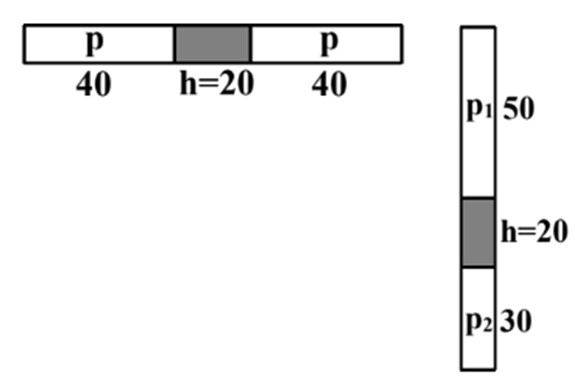
\includegraphics[width=0.35\linewidth]{figs/VN12-Y24-PH-SYL-010P-5}
		\end{center}
		Theo định luật Boyle:
		$$\begin{cases}
			p\cdot40 S=p_1\cdot50S\\
			p\cdot40S=p_2\cdot30S
		\end{cases}\Rightarrow \begin{cases}
			p_1=0,8p\\
			p_2=\dfrac{4p}{3}
		\end{cases}$$
		Khi đặt ống thẳng đứng thì cột thuỷ ngân cân bằng khi:
		$$p_2=p_1+h\Rightarrow p=\SI{37.5}{\centi\meter Hg}.$$
	}
\end{ex}
% ===================================================================
\begin{ex}
	Một ống hình trụ hẹp, kín hai đầu, dài $\ell=\SI{105}{\centi\meter}$, đặt nằm ngang. Chính giữa ống có một cột thuỷ ngân dài $h=\SI{21}{\centi\meter}$, phần còn lại của ống chứa không khí ở áp suất $p_0=\SI{72}{\centi\meter Hg}$. Coi nhiệt độ không khí trong ống không thay đổi. Khi ống đặt thẳng đứng thì độ di chuyển của cột thuỷ ngân là
	\choice
	{$\SI{3}{\centi\meter}$}
	{$\SI{4}{\centi\meter}$}
	{\True $\SI{6}{\centi\meter}$}
	{$\SI{2}{\centi\meter}$}
	\loigiai{$$pV=\text{const}\Rightarrow \begin{cases}
			72\cdot42=p_1\left(42+x\right)\\
			72\cdot42=p_2\left(42-x\right)
		\end{cases}\Rightarrow \begin{cases}
			p_1=\dfrac{3024}{42+x}\\
			\ \\
			p_2=\dfrac{3024}{42-x}
		\end{cases}.$$
		Mà
		$$p_2=p_1+h\Rightarrow x=\SI{6}{\centi\meter}.$$
	}
\end{ex}
% ===================================================================
\begin{ex}
	\immini{
	Một lượng không khí có thể tích $\SI{240}{\centi\meter^3}$ chứa trong một cylanh có piston đóng kín, tiết diện của piston là $\SI{24}{\centi\meter^2}$. Áp suất của không khí trong cylanh bằng áp suất không khí bên ngoài và bằng $\SI{100}{\kilo\pascal}$. Cần một lực bằng bao nhiêu để dịch chuyển piston $\SI{2}{\centi\meter}$ theo chiều làm thể tích khí giảm? Bỏ qua ma sát giữa piston và thành cylanh. Coi trong quá trình chuyển động nhiệt độ khí không đổi.

}{
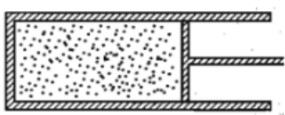
\includegraphics[scale=0.5]{figs/VN12-Y24-PH-SYL-010P-3}
}
	\choice
{$\SI{20}{\newton}$}
{$\SI{80}{\newton}$}
{\True $\SI{60}{\newton}$}
{$\SI{40}{\newton}$}
	
	\loigiai{\begin{center}
			\begin{tabular}{C{4cm} C{3cm} C{4cm}}
				\colorbox{yellow}{\textcolor{red}{\textbf{Trạng thái 1}}} & $\xrightarrow[]{T_1=T_2}$ & \colorbox{yellow}{\textcolor{red}{\textbf{Trạng thái 2}}}\\
				$p_1=\SI{100}{\kilo\pascal}$ & &$p_2=?$\\
				$V_1=\SI{240}{\centi\meter^3}$ & & $V_2=\SI{192}{\centi\meter^3}$
			\end{tabular}
		\end{center}
		Theo định luật Boyle:
		$$p_1V_1=p_2V_2\Rightarrow p_2=\SI{125}{\kilo\pascal}.$$
		Piston cân bằng khi:
		$$F+p_0S=p_2S\Rightarrow F=\left(p_2-p_0\right)S=\SI{60}{\newton}.$$
	}
\end{ex}
% ===================================================================
\begin{ex}
	Một bơm xe đạp hình trụ có đường kính trong là $\SI{3}{\centi\meter}$. Người ta dùng ngón tay bịt kín đầu vòi bơm và ấn piston từ từ để nén không khí trong bơm sao cho nhiệt độ không thay đổi. Lấy áp suất khí quyển là $p_0=\SI{E5}{\pascal}$. Để thể tích của không khí trong bơm giảm đi 4 lần thì lực tác dụng lên piston là
	
	\choice
	{$\SI{250}{\newton}$}
	{$\SI{225}{\newton}$}
	{$\SI{200}{\newton}$}
	{\True $\SI{212}{\newton}$}
	\loigiai{Theo định luật Boyle:
		$$p_0V_0=p\dfrac{V_0}{4}\Rightarrow p=4p_0.$$
		Để piston cân bằng:
		$$F+p_0S=pS\Rightarrow F=\left(p-p_0\right)S=3p_0\cdot\pi\dfrac{d^2}{4}\approx\SI{212}{\newton}.$$
	}
\end{ex}
% ===================================================================
\begin{ex}
	\immini{
Cylanh và piston nhẹ cách nhiệt chứa bên trong nó một lượng khí xác định. Ban đầu thể tích khí chứa trong cylanh là $\SI{1000}{\centi\meter^3}$. Tiến hành đặt lên piston một gia trọng có khối lượng $\SI{10}{\kilogram}$. Biết tiết diện của piston là $S=\SI{100}{\centi\meter^2}$, lấy $g=\SI{10}{\meter/\second^2}$, áp suất khí quyển $p_0=\SI{E5}{\pascal}$. Thể tích của khí trong cylanh khi piston cân bằng là

}{
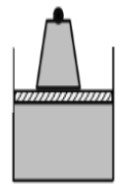
\includegraphics[scale=0.6]{figs/VN12-Y24-PH-SYL-010P-4}
}
\choice
{\True $\SI{910}{\centi\meter^3}$}
{$\SI{1100}{\centi\meter^3}$}
{$\SI{800}{\centi\meter^3}$}
{$\SI{600}{\centi\meter^3}$}	
	\loigiai{\begin{center}
			\begin{tabular}{C{4cm} C{3cm} C{4cm}}
				\colorbox{yellow}{\textcolor{red}{\textbf{Trạng thái 1}}} & $\xrightarrow[]{T_1=T_2}$ & \colorbox{yellow}{\textcolor{red}{\textbf{Trạng thái 2}}}\\
				$p_1=\SI{E5}{\pascal}$ & &$p_2=p_0+\dfrac{mg}{S}=\SI{1.1E5}{\pascal}$\\
				$V_1=\SI{1000}{\centi\meter^3}$ & & $V_2=?$
			\end{tabular}
		\end{center}
		Theo định luật Boyle:
		$$p_1V_1=p_2V_2\Rightarrow V_2\approx\SI{910}{\centi\meter^3}.$$
	}
\end{ex}
% ===================================================================
\begin{ex}
Ở chính giữa một ống thuỷ tinh nằm ngang, kín cả hai đầu có một cột thuỷ ngân dài $h=\SI{19.6}{\centi\meter}$. Nếu đặt ống nghiêng một góc $\SI{30}{\degree}$ so với phương nằm ngang thì cột thuỷ ngân dịch chuyển một đoạn $\Delta \ell_1=\SI{20}{\milli\meter}$. Nếu đặt ống thẳng đứng thì cột thuỷ ngân dịch chuyển một đoạn $\Delta \ell_2=\SI{30}{\milli\meter}$. Coi nhiệt độ không khí không thay đổi. Áp suất của không khí trong ống khi ống nằm ngang gần bằng
	
	\choice
	{$\SI{19}{\milli\meter Hg}$}
	{$\SI{6}{\milli\meter Hg}$}
	{\True $\SI{10}{\milli\meter Hg}$}
	{$\SI{30}{\milli\meter Hg}$}
	\loigiai{\begin{center}
			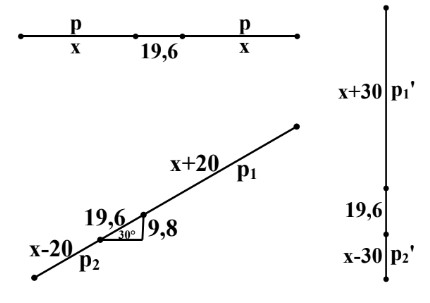
\includegraphics[width=0.35\linewidth]{figs/VN12-Y24-PH-SYL-010P-6}
		\end{center}
		Theo định luật Boyle:
		$$pV=\text{const}\Rightarrow \begin{cases}
			px=p_1\left(20+x\right)=p'_1\left(30+x\right)\\
			px=p_2\left(x-20\right)=p'_2\left(x-30\right)
		\end{cases}$$
		Lại có
		$$\begin{cases}
			p_2=p_1+19,6\sin\SI{30}{\degree}\\
			p'_2=p'_1+19,6
		\end{cases}\Rightarrow \begin{cases}
			p_2-p_1=9,8\\
			p'_2-p'_1=19,6
		\end{cases}$$
		$$\Rightarrow\begin{cases}
			\dfrac{px}{x-20}-\dfrac{px}{x+20}=9,8\\
			\ \\
			\dfrac{px}{x-30}-\dfrac{px}{x+30}=19,6
		\end{cases}\Rightarrow \begin{cases}
			p\approx\SI{10}{\milli\meter Hg}\\
			x\approx\SI{48.99}{\milli\meter}
		\end{cases}.$$
	}
\end{ex}
% ===================================================================
\begin{ex}
	\immini{
	Một ống thuỷ tinh được cắm lộn ngược vào một chậu thuỷ ngân, bên trong ống chứa $\SI{40}{\centi\meter^3}$ không khí và một cột thuỷ ngân cao $\SI{8}{\centi\meter}$ so với mực thuỷ ngân trong chậu (hình a). Người ta ấn sâu ống thuỷ tinh vào thuỷ ngân cho tới khi mực thuỷ ngân ở bên trong và bên ngoài ống bằng nhau (hình b). Biết áp suất khí quyển là $\SI{75}{\centi\meter Hg}$. Xem nhiệt độ không khí trong ống không thay đổi. Thể tích của không khí còn lại bên trong ống lúc sau là
}
{
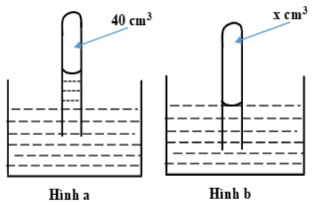
\includegraphics[scale=0.6]{figs/VN12-Y24-PH-SYL-010P-7}
}
\choice
{$\SI{44.78}{\centi\meter^3}$}
{$\SI{35.7}{\centi\meter^3}$}
{$\SI{44.27}{\centi\meter^3}$}
{$\SI{36.14}{\centi\meter^3}$}
	\loigiai{\begin{center}
			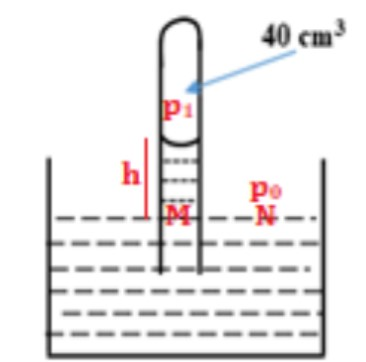
\includegraphics[width=0.2\linewidth]{figs/VN12-Y24-PH-SYL-010P-8}
		\end{center}
		Hình a có áp suất tại hai điểm M và N trên mặt phẳng nằm ngang bằng nhau:
		$$p_\text{M}=p_\text{N}\Rightarrow p_1+h=p_0\Rightarrow p_1=p_0-h=\SI{67}{\centi\meter Hg}.$$
		Tương tự ở hình b có $p_2=p_0=\SI{75}{\centi\meter Hg}$.\\
		Theo định luật Boyle:
		$$p_1V_1=p_2V_2\Rightarrow V_2\approx\SI{35.7}{\centi\meter^3}.$$}
\end{ex}
\Closesolutionfile{ans}

